%
\section{System overview}
\label{sec:system-overview}
The system overview presents a global view of the system, considering its main
features, components and interactions. It is not intended to be complete, but
rather provide a basis for the outline of the system architecture.
Fig.~\ref{fig:sys-overview} presents the \gls{mdo} system overview.
%
\begin{figure}[htb!]
\centering
    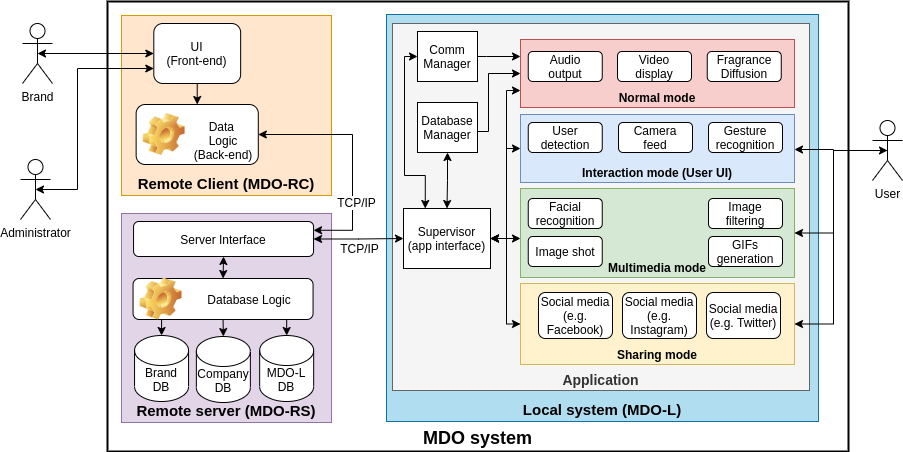
\includegraphics[width=1.0\columnwidth]{./img/sys-overview.png}
  \caption{\gls{mdo} system overview}%
\label{fig:sys-overview}
\end{figure}

Considering the system interactions, three main actors were identified:
\begin{enum-c}
\item \emph{Brand}: represents the brands contracting the advertisement
  services;
\item \emph{Administrator}: the development company staff, which can monitor and
  control the outdoor (administrative privileges).
\item \emph{User}: the user (the target audience of the advertisement)
  interacting with the system.
\end{enum-c}

Considering the data flow across the \textbf{MDO system}, three main subsystems were
identified: \textbf{\gls{mdo-rc}}, \textbf{\gls{mdo-rs}}, and
\textbf{\gls{mdo-l}}. The rational behind this initial decomposition is
explained next.

\subsection{MDO Remote Client}
The \emph{Brand} and \emph{Administrator} members require a remote \gls{ui} (front-end) to
interact with the system: the former to configure the advertisements being
displayed at the \gls{mdo} and purchase them; the latter to remotely monitor and
control the operation of the \gls{mdo}. Thus, it is clear that \emph{an
  authentication mechanism must be provided for the remote \gls{ui}}.

The data is then dispatched to the back-end, where it is processed and feed back
to the \gls{ui} user and/or sent to the remote server, via \gls{tcp-ip}
comprising the data logic component of the \gls{ui}.
%
%
\subsection{MDO Remote Server}
\label{sec:mdo-remote-server}
Although the \gls{mdo-rc} could communicate directly with the \gls{mdo-l}, this
is not desirable or a good architecture mainly due to: communications failure could
result in data loss, compromising the system's integrity; the remote client and
the local system become tightly coupled, meaning the remote client must be aware
of all the available local systems; if the data storage in the local system
fails, the remote client would have to provide the backup information.

Thus, a remote server component is included, providing the access and management
of the system databases, pertaining to the \emph{Brand}, \emph{Company}, and
\emph{MDO Local system}. The first two provide the historical information of the
\texttt{Brand} and \texttt{Administrator} entities, and the last one the information
related to all of the \texttt{\gls{mdo-l}} systems in operation.

The main functions of the \texttt{\gls{mdo-rs}} are:
\begin{item-c}
\item \emph{UI requests responses}: when a \gls{ui} user requests/modifies
  some information from the database, the server must provide/update it.
\item \emph{\gls{mdo-l} monitoring and control}: provide command dispatch and
  feedback to the \texttt{Administrator} staff for remote monitoring and control of
  the device.
\item \emph{\gls{mdo-l} update}: periodically check for start times of each
  \gls{mdo-l} device and transfer the relevant data to it.
\end{item-c}

The server interface is the responsible for managing the requests and respective
responses from the remote client and for periodically send the update data to
all \gls{mdo-l} devices. 
%
%
\subsection{MDO Local system}
\label{sec:mdo-local-system}
The \gls{mdo} local system (MDO-L) is the marketing device, interacting with the user
to display multi-sensory advertisements. As aforementioned in
Section~\ref{sec:prob-stat}, it is comprised of four modes:
\begin{item-c}
\item \emph{normal mode}: the MDO provides sound, video and fragrance
  outputs. It is the default mode.
\item \emph{interaction mode}: When a user approaches the device, the \gls{mdo} will
go into interaction mode, turning on and displaying the camera feed and waiting
for recognizable gestures to provide additional functionalities, such as
brand-specific image filters. This is the \texttt{User} \gls{ui}.
\item \emph{multimedia mode}: in this mode the facial detection is applied,
  enabling the user to select and apply different brand-specific image filters and take pictures or create a \gls{gif}.
\item \emph{sharing mode}: after a user take a picture or create a \gls{gif}, it
  can share it across social media.
\end{item-c}

The user interaction is considered to be a higher priority activity than the
advertisements, so when a \texttt{User} interacts with the system, the \texttt{normal
mode} is overriden by the \texttt{Interaction mode}, thus, halting the
advertisements.

The \gls{mdo-l} application communicates with the remote server
(\texttt{\gls{mdo-rs}}) through the \texttt{Supervisor} via \gls{tcp-ip}
 to handle requests from \texttt{Administrator} members
to monitor and control the device through the \texttt{Supervisor} or to update
the advertisements. Additionally, the \texttt{Supervisor} oversees the
application mode and the communication (\texttt{Comm Manager}) and database
(\texttt{Database manager}) managers to handle system events.
%
%%% Local Variables:
%%% mode: latex
%%% TeX-master: "../../../dissertation"
%%% End:
